\documentclass[tikz,border=4pt]{standalone}
\usepackage{amsmath}
\begin{document}
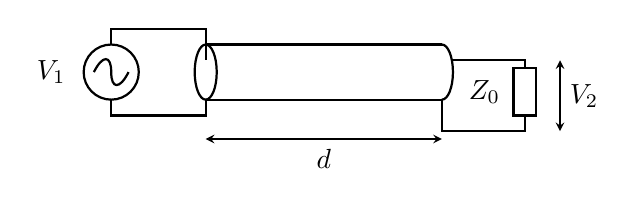
\begin{tikzpicture}[>=stealth, thick, scale=1.0]
  % AC source on left
  \draw[thick] (-0.9, 0) circle (0.35);
  \draw[thick] (-1.12, 0) .. controls (-1.01, 0.22) and (-0.90, 0.22) .. (-0.90, 0)
               .. controls (-0.90, -0.22) and (-0.79, -0.22) .. (-0.68, 0);
  \node[left] at (-1.35, 0) {$V_1$};

  % Connections left
  \draw[thick] (-0.9, 0.35) -- (-0.9, 0.55) -- (0.3, 0.55) -- (0.3, 0.15);
  \draw[thick] (-0.9, -0.35) -- (-0.9, -0.55) -- (0.3, -0.55) -- (0.3, -0.35);

  % Coaxial cable body of length d
  \draw[thick] (0.3, 0.35) -- (3.3, 0.35);
  \draw[thick] (0.3, -0.35) -- (3.3, -0.35);
  \draw[thick] (0.3, 0) ellipse (0.14 and 0.35);
  \draw[thick] (3.3, 0.35) arc (90:-90:0.14 and 0.35);

  % Length d indicator
  \draw[<->, thin] (0.3, -0.85) -- (3.3, -0.85) node[midway, below] {$d$};

  % Termination resistor Z_0 on right (wider gap from cylinder)
  \draw[thick] (3.44, 0.15) -- (4.35, 0.15) -- (4.35, 0.05);
  \draw[thick] (4.21, 0.05) rectangle (4.49, -0.55);
  \node[left] at (4.17, -0.25) {$Z_0$};
  \draw[thick] (4.35, -0.55) -- (4.35, -0.75) -- (3.3, -0.75) -- (3.3, -0.35);

  % Output voltage V_2
  \draw[<->, thin] (4.80, 0.15) -- (4.80, -0.75) node[midway, right] {$V_2$};
\end{tikzpicture}
\end{document}
